\scanpage{233}
\mspage{183}
% L1
\[
E_2^{pq}\xrightarrow{\sim}E^{\prime pq}_2\qquad\text{iso si }q\leq n
\tag*{($\alpha$)}
\]
% L2
Dans le cas $n=2$, utilisant que
% L3
\[
E_2^{p1}=E^{\prime p1}_2=0\qquad\text{car }H^1(\widetilde X)=H^1(\widetilde Y)=0,
\]
% L4
on trouve deux suites exactes
% L3–4, right
\figure{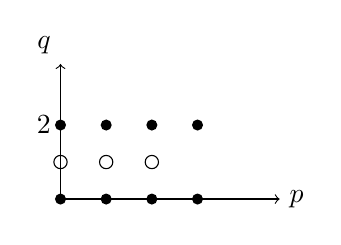
\begin{tikzpicture}[x=.58cm,y=.47cm]
\draw[->] (0,0)--(4.8,0) node[right] {$p$};
\draw[->] (0,0)--(0,3.65) node[above left] {$q$};
\node[left] at (0,2) {$2$};
\foreach \x in {0,1,2,3}{\fill (\x,0) circle (2pt); \fill (\x,2) circle (2pt);}
\foreach \x in {0,1,2}{\draw (\x,1) circle (2.4pt);}
\end{tikzpicture}}
% L5–7
\diagram{\begin{tikzcd}[ampersand replacement=\&,column sep=tiny,row sep=large]
\unsure{\cdot|0}\arrow[r] \& H^2(\pi,H^0(\widetilde Y))\arrow[r]\arrow[d,"\mathrm{iso}"] \& H^2(Y)\arrow[r]\arrow[d] \& H^0(\pi,H^2(\widetilde Y))\arrow[r]\arrow[d,"\mathrm{iso}"] \& H^3(\pi,H^0(\widetilde Y))\arrow[d,"\mathrm{iso}"]\\
0\arrow[r] \& H^2(\pi,H^0(\widetilde X))\arrow[r] \& H^2(X)\arrow[r] \& H^0(\pi,H^2(\widetilde X))\arrow[r] \& H^3(\pi,H^0(\widetilde Y))
\end{tikzcd},}
% L8–10
et un hom de l'une dans l'autre, qui permet de conclure par le lemme des 5 que $H^2(Y;F)\to H^2(X,F_{\unsure{x|X}})$ est iso.
% L10–16
Mais pour $n$ quelconque, la relation ($\alpha$) sur les termes $E_2$ \inserted{(pour $q\leq n$)} ne me semble pas impliquer la relation similaire pour les $E_r$ supérieurs, et de là pour les termes $E_\infty$, ce qui permettrait de conclure\unsure{.}

% L17–19
Je reviens donc à la suite exacte p. \unsure{187|181}, avec $F$ faisceau \uline{tordu}. J'ai envie de trouver une application canonique
% L20
\[
H^n(X,\unsure{G|E|\mathcal G})\longrightarrow\overbrace{\mathrm{Hom}_{\pi}(\pi_n(X,x),G_x)}^{\inserted{\substack{\text{Hom \uline{additifs} bien sûr}\\\text{i.e. en }\mathbb Z[\pi]\text{-modules}}}}, 
\]
% L21–22
où $G$ est un faisceau abélien loc. constant \unsure{quelc.} sur $X$, et $\pi=\pi_1(X,x)$. Si j'interprète
% archive sheet number: 233
